\documentclass[11pt,a4paper,pdftex]{article}
\usepackage{longtable}
\usepackage{multirow}
\usepackage{pdfpages}
\usepackage{float}

% Language setting % Replace `english' with e.g. `spanish' to change the document language
\usepackage[english]{babel}

% Set page size and margins
% Replace `letterpaper' with `a4paper' for UK/EU standard size
\usepackage[letterpaper,top=2cm,bottom=2cm,left=3cm,right=3cm,marginparwidth=1.75cm]{geometry}

% Useful packages
\usepackage{amsmath}
\usepackage[hidelinks]{hyperref}
\usepackage{graphicx}
\usepackage{csquotes}
\usepackage{indentfirst}
\usepackage{parskip}
\graphicspath{{/graphics/}}

\begin{document}

% ----- Title Page -----
\begin{titlepage}
    \centering
    \vspace*{2cm}
    
\includegraphics[scale=0.7]{graphics/vu mif.png}

    
    {\Large \textbf{Vilnius University}}\\[0.5cm]
    {\large Mathematics and Informatics Faculty}\\[0.3cm]
    {\large Software Engineering study program, III course}\\[3cm]
    
    {\Huge \textbf{PoS System Software Design Document}}\\[3cm]
    
    \begin{flushleft}
    Viktorija Šimonėlytė 4 gr. \\
    Artiom Garbul 2 gr. \\
    Mykolas M. Budrys 2 gr. \\
    Elvinas Švilpa 4 gr. \\
    Artūras Mecelis 4 gr. \\
    \end{flushleft}
    
    \vfill

    \textit{Version: 1.0}

    \vspace{1em}
    
    {\large \today}
\end{titlepage}

\tableofcontents
\newpage

\section{Introduction}

This document provides detailed documentation of a Point of Sale (POS) system designed specifically for small to medium-sized catering and beauty businesses. The platform centralizes customer order management, supports scheduling and handling of appointments and provides a universal software-based service suitable for a wide range of day-to-day business operational needs.

\section{Business flows}
\subsection{Practical business flow examples}
To start of with building a POS system, practical examples as to the possible business flows are required.

\subsubsection{Restaurant Order Business Flow}
The restaurant order flow (Figure \ref{figures:sequence_restaurant}) illustrates the customer experience within a restaurant setting. The waiter uses the POS system to confirm reservations, check for available tables, and mark occupied tables. All orders are registered through the POS system, which also sends order information to the kitchen staff.

Once the meals are ready, the POS system notifies the waiter to deliver the food to the customer. The system also accommodates additional orders during the visit. At checkout, the POS system generates an itemized receipt, supports split billing, registers payments, and records tips. The order is then finalized and marked as complete. 

% pridėti pavadinimus 
A practical example involving a walk-in customer order:

\begin{figure}[H]
    \centering
    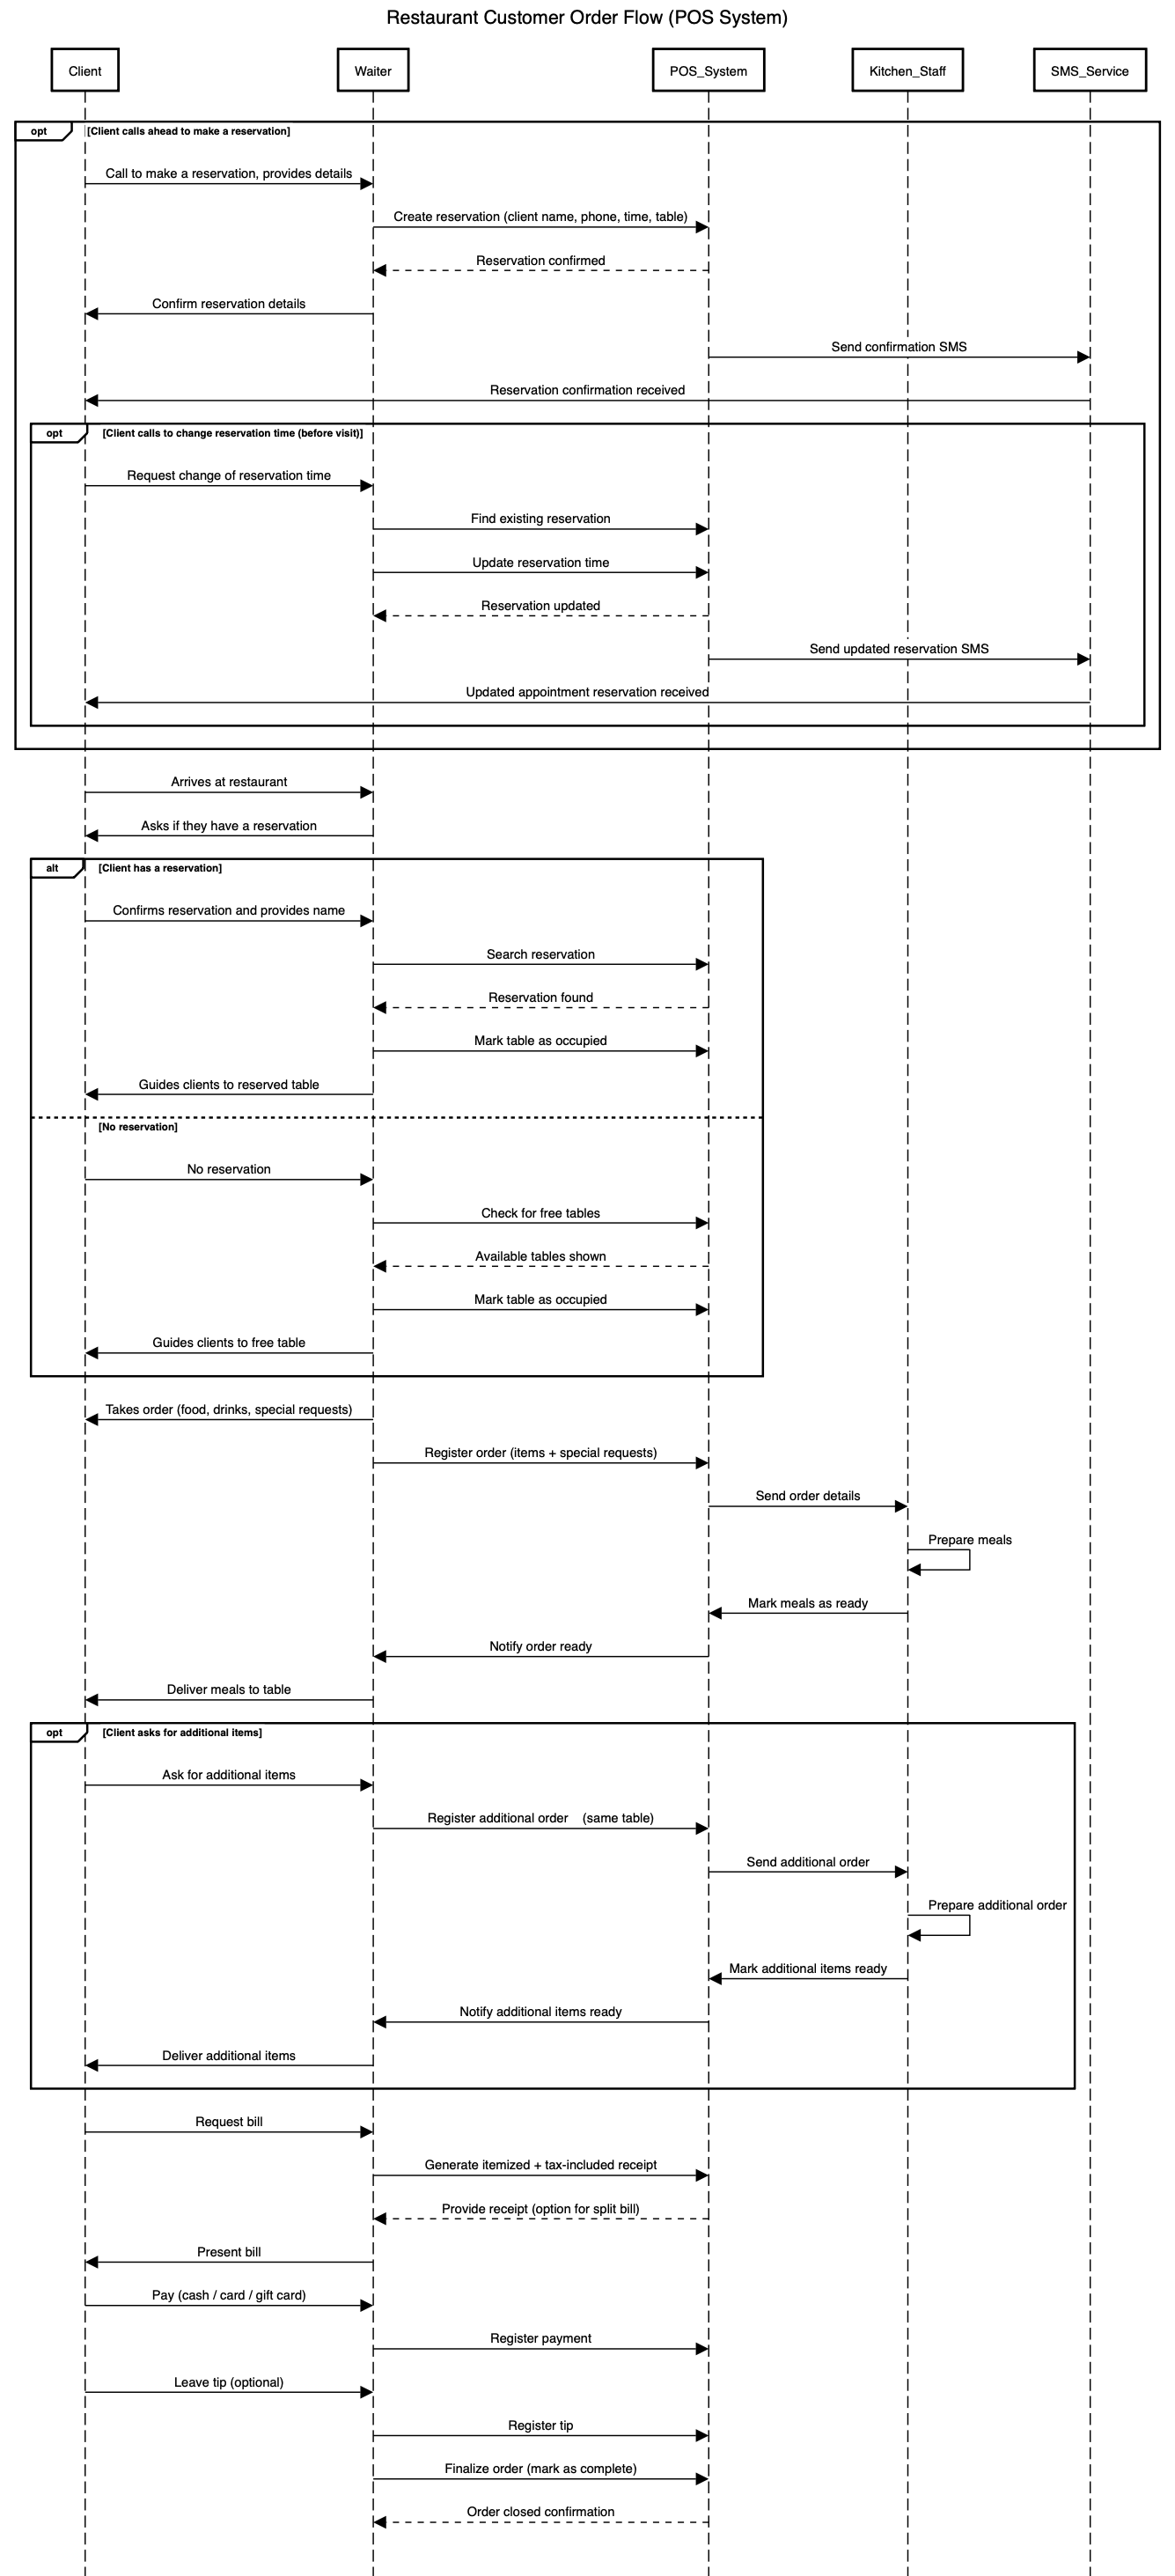
\includegraphics[scale=0.22]{graphics/restaurant.png}
    \caption{Sequence diagram displaying possible business actions in a restaurant}
    \label{figures:sequence_restaurant}
\end{figure}
% 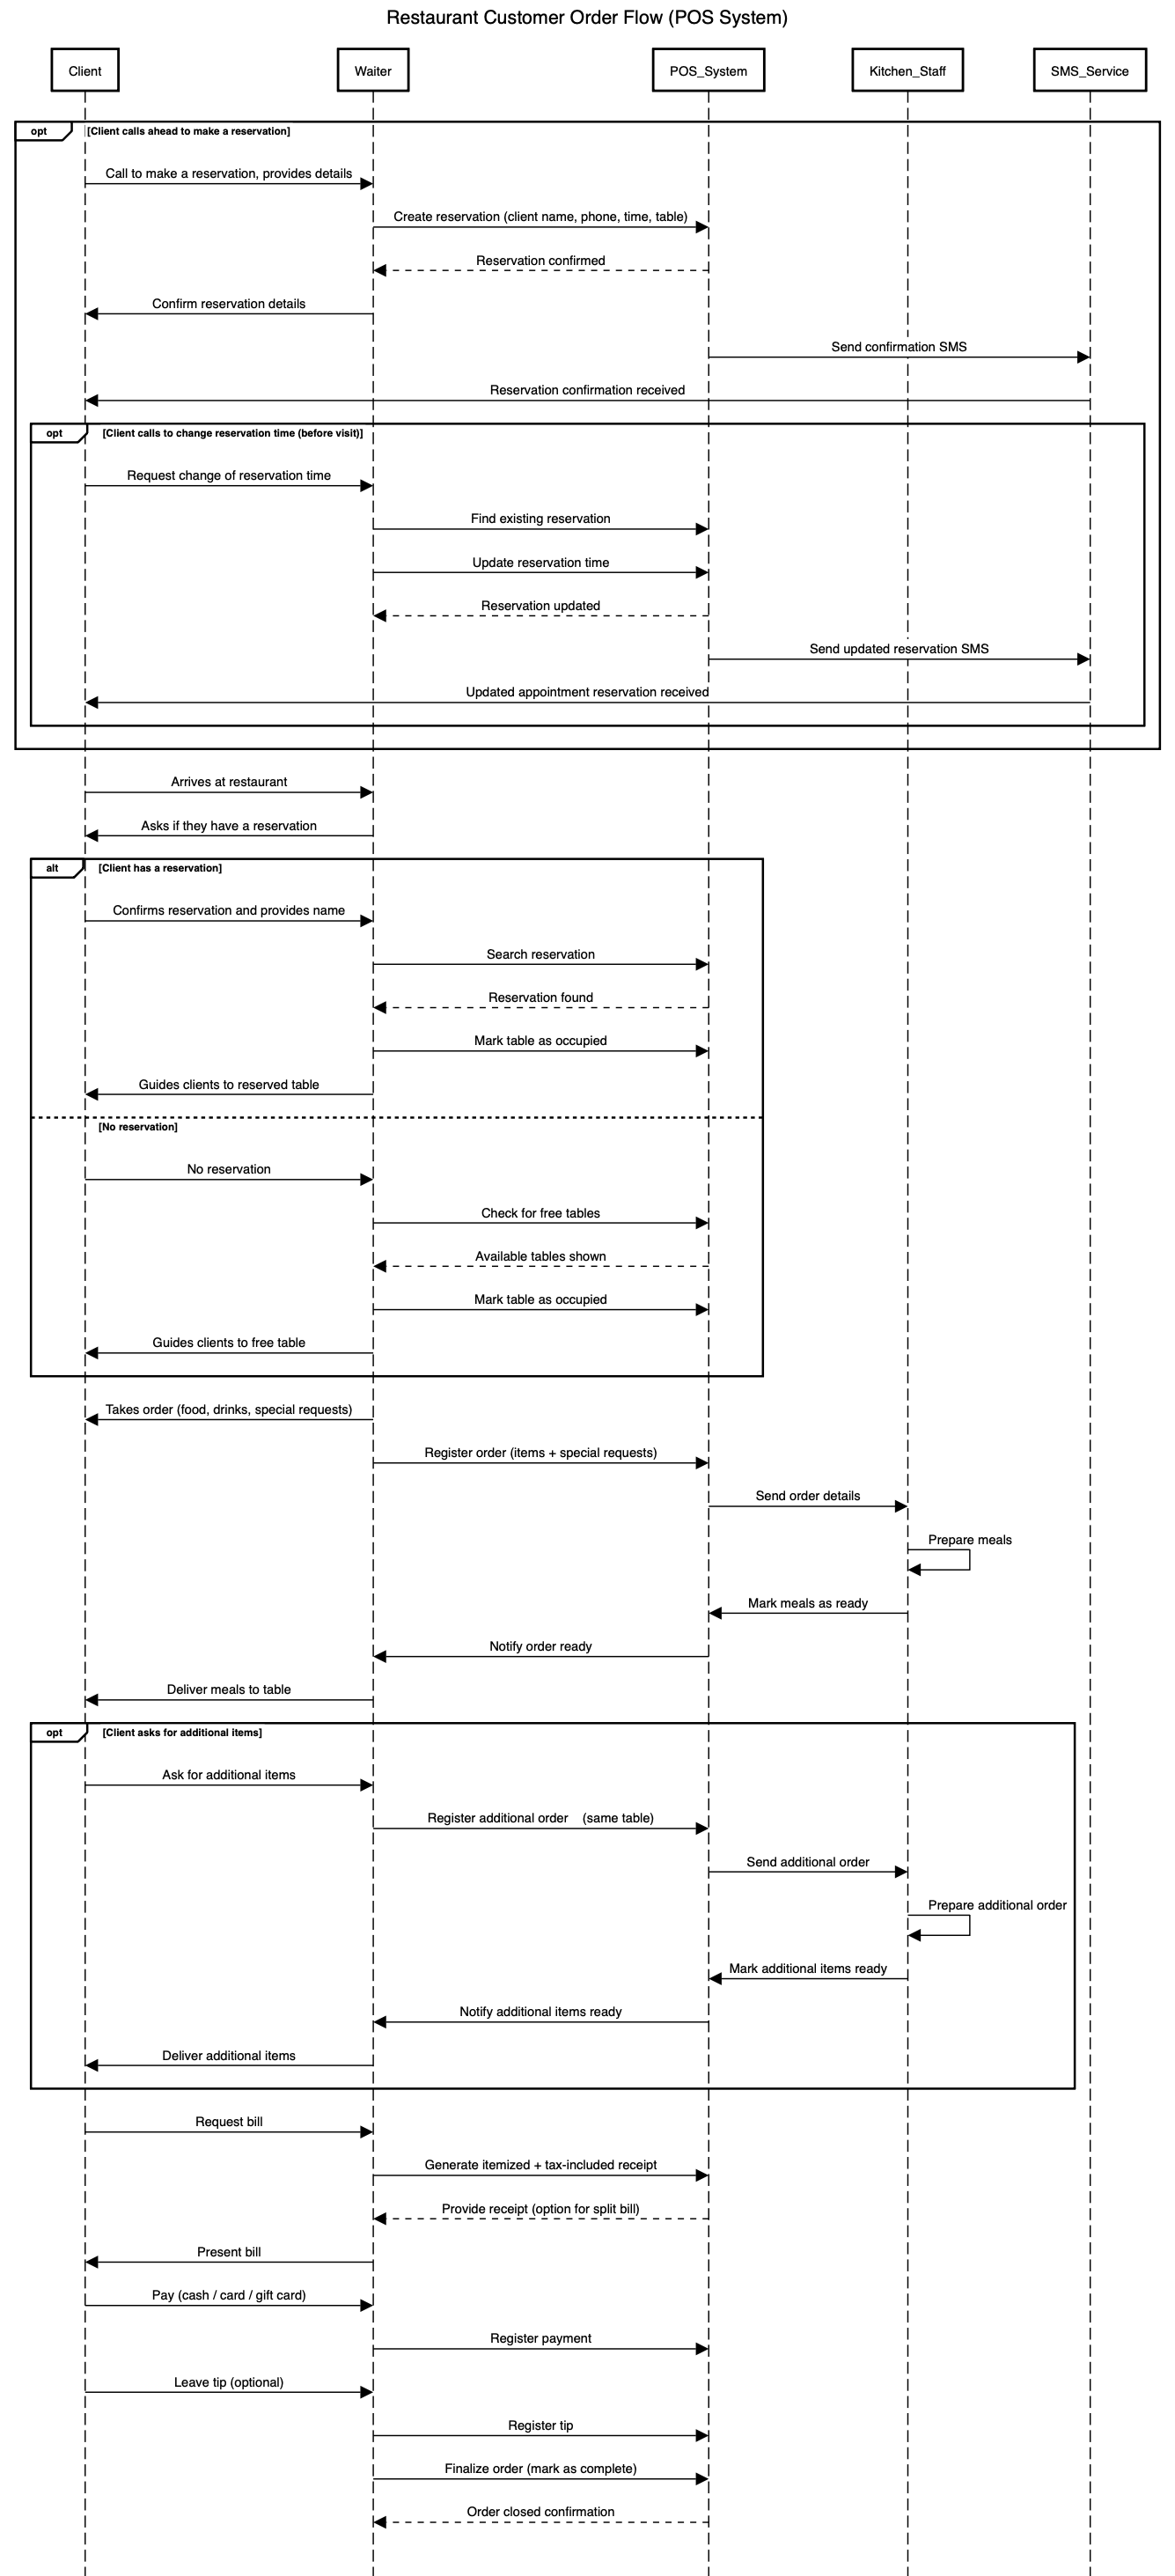
\includepdf[pages=-,scale=0.95]{graphics/restaurant.png}

\subsubsection{Beauty Salon Appointment Business Flow}

The beauty salon appointment flow (Figure \ref{figures:sequence_beauty_salon}) focuses on how client appointments are handled with the POS system. The receptionist creates or updates the appointment in the POS system at the request of a client. These appointments send confirmation messages via an SMS service. Once the client has arrived, the reservation is checked and order for the services created. Walk-in clients can also select their desired service and time slot based on available options. 

After such services are completed, payment process is initiated - the POS system generates an itemized receipt, applies discounts if available, registers tips, processes payment and marks the order as complete.

An example of a beauty salon appointment:

\begin{figure}[H]
    \centering
    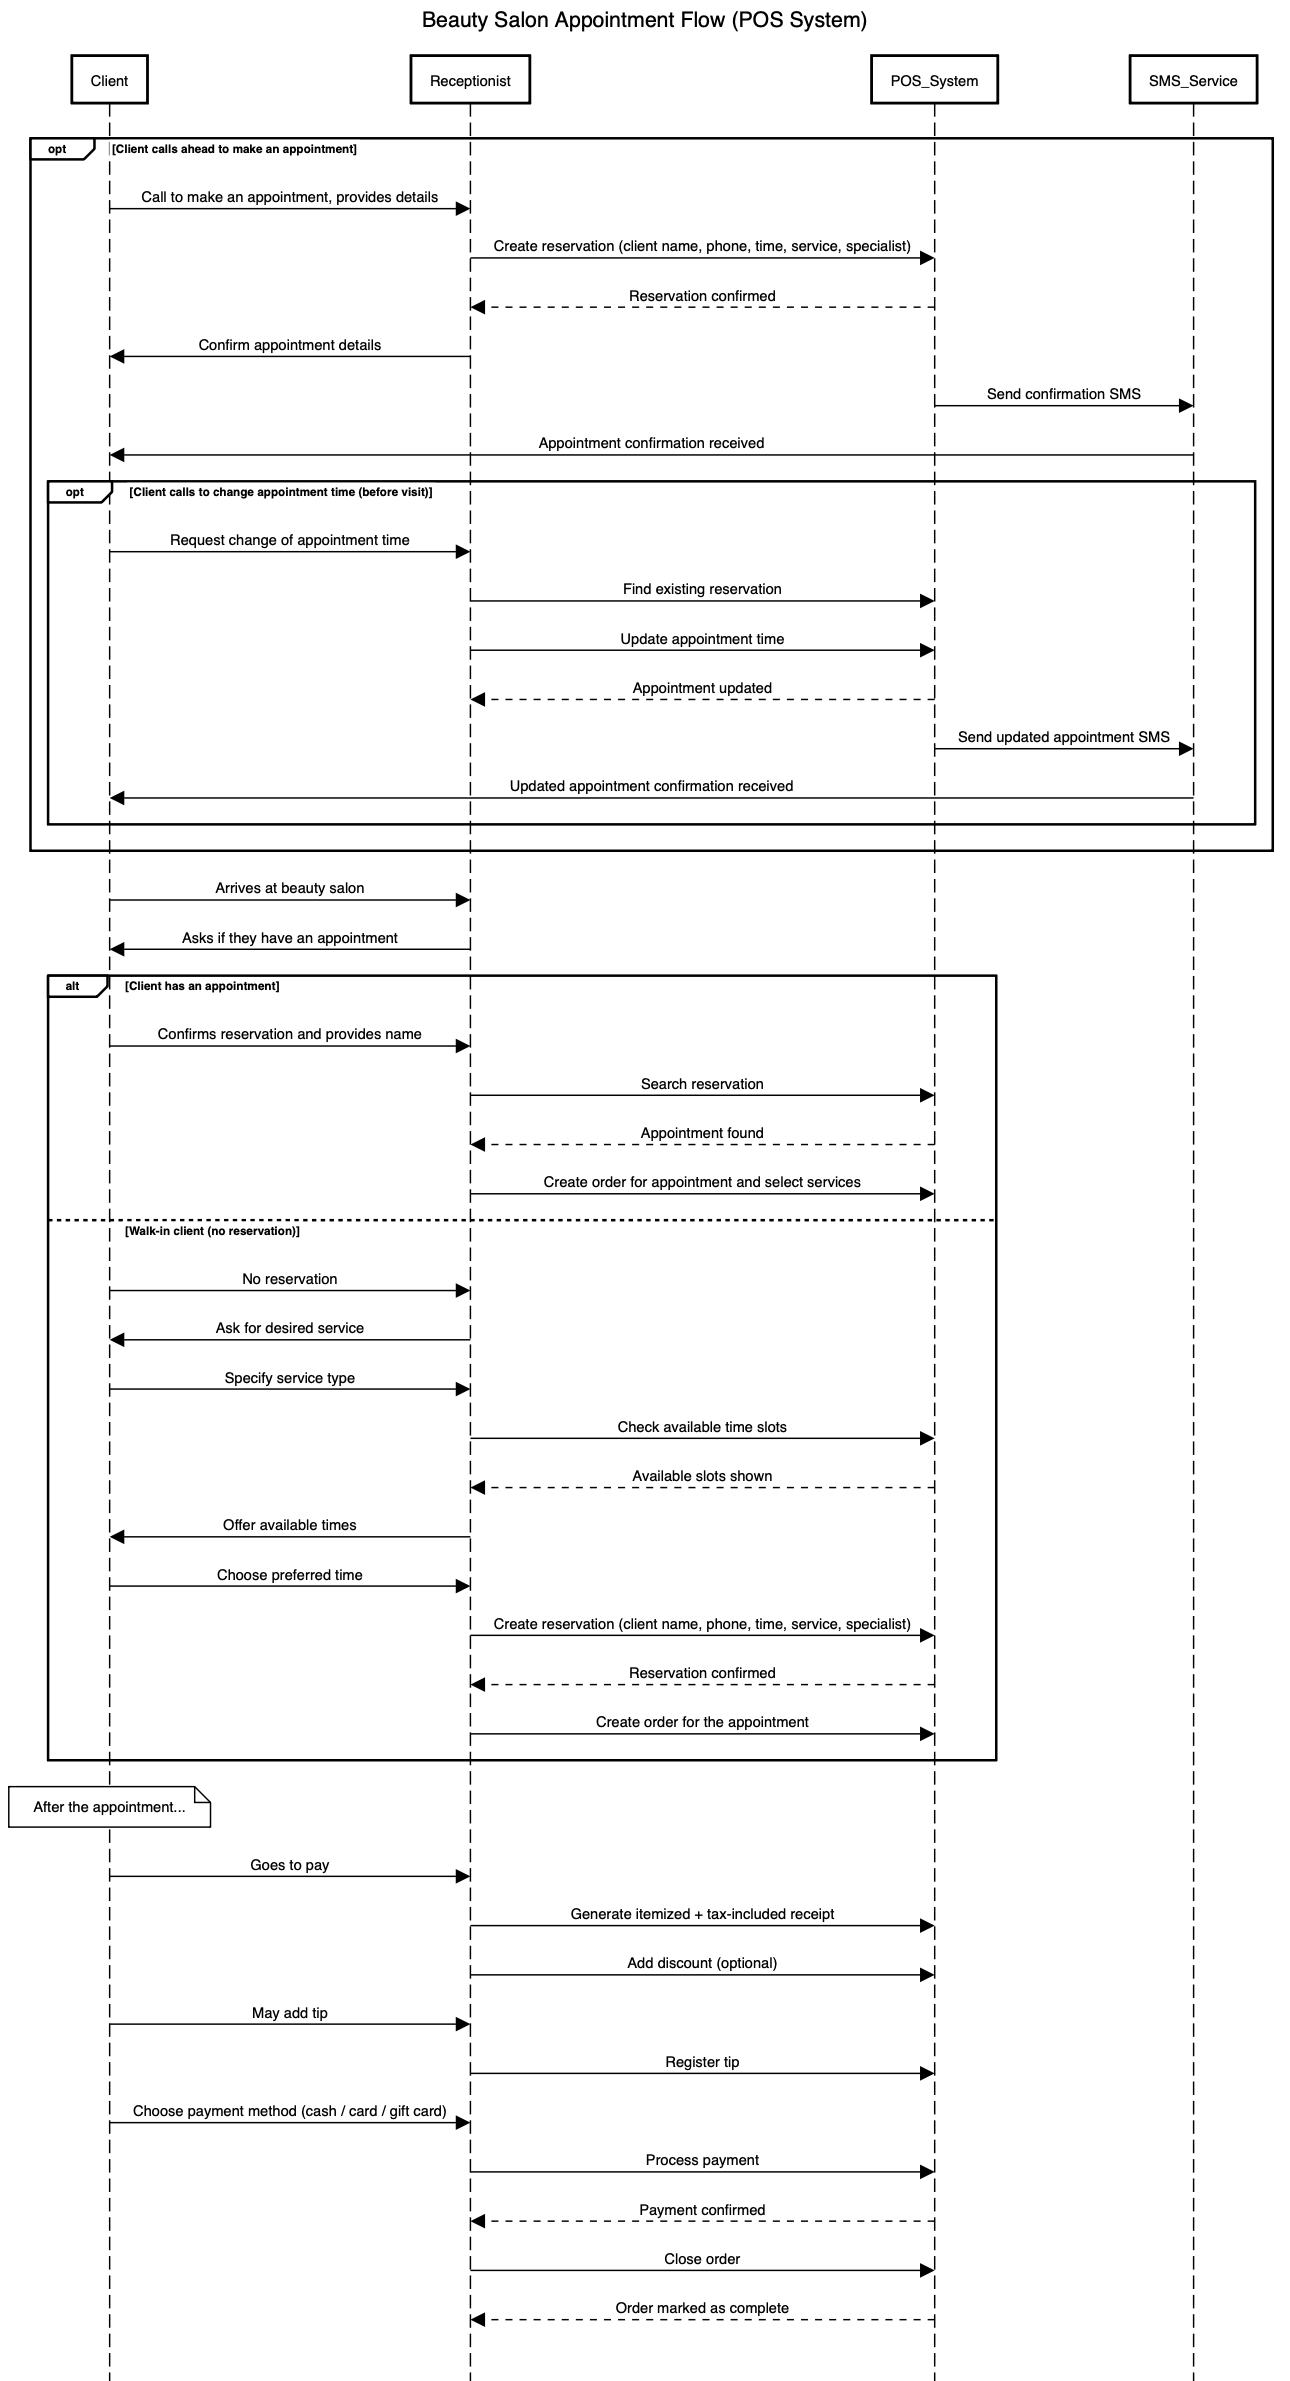
\includegraphics[scale=0.22]{graphics/beauty salon.png}
    \caption{Sequence diagram displaying possible business actions in a beauty salon}
    \label{figures:sequence_beauty_salon}
\end{figure}


\subsubsection{Business Owner Management Business Flow}

The business owner business flow (Figure \ref{figures:sequence_business_owner}) depicts how business owners interact with the POS system to manage their business operations. After logging in, owners access the management dashboard to handle administrative tasks such as managing inventory, taxes, discounts and more. Additionally, owners can manage user accounts, update business details. 
SuperAdmin intervention is also supported, allowing oversight and configuration when necessary. 

An example of a business owner configuring the system:

\begin{figure}[H]
    \centering
    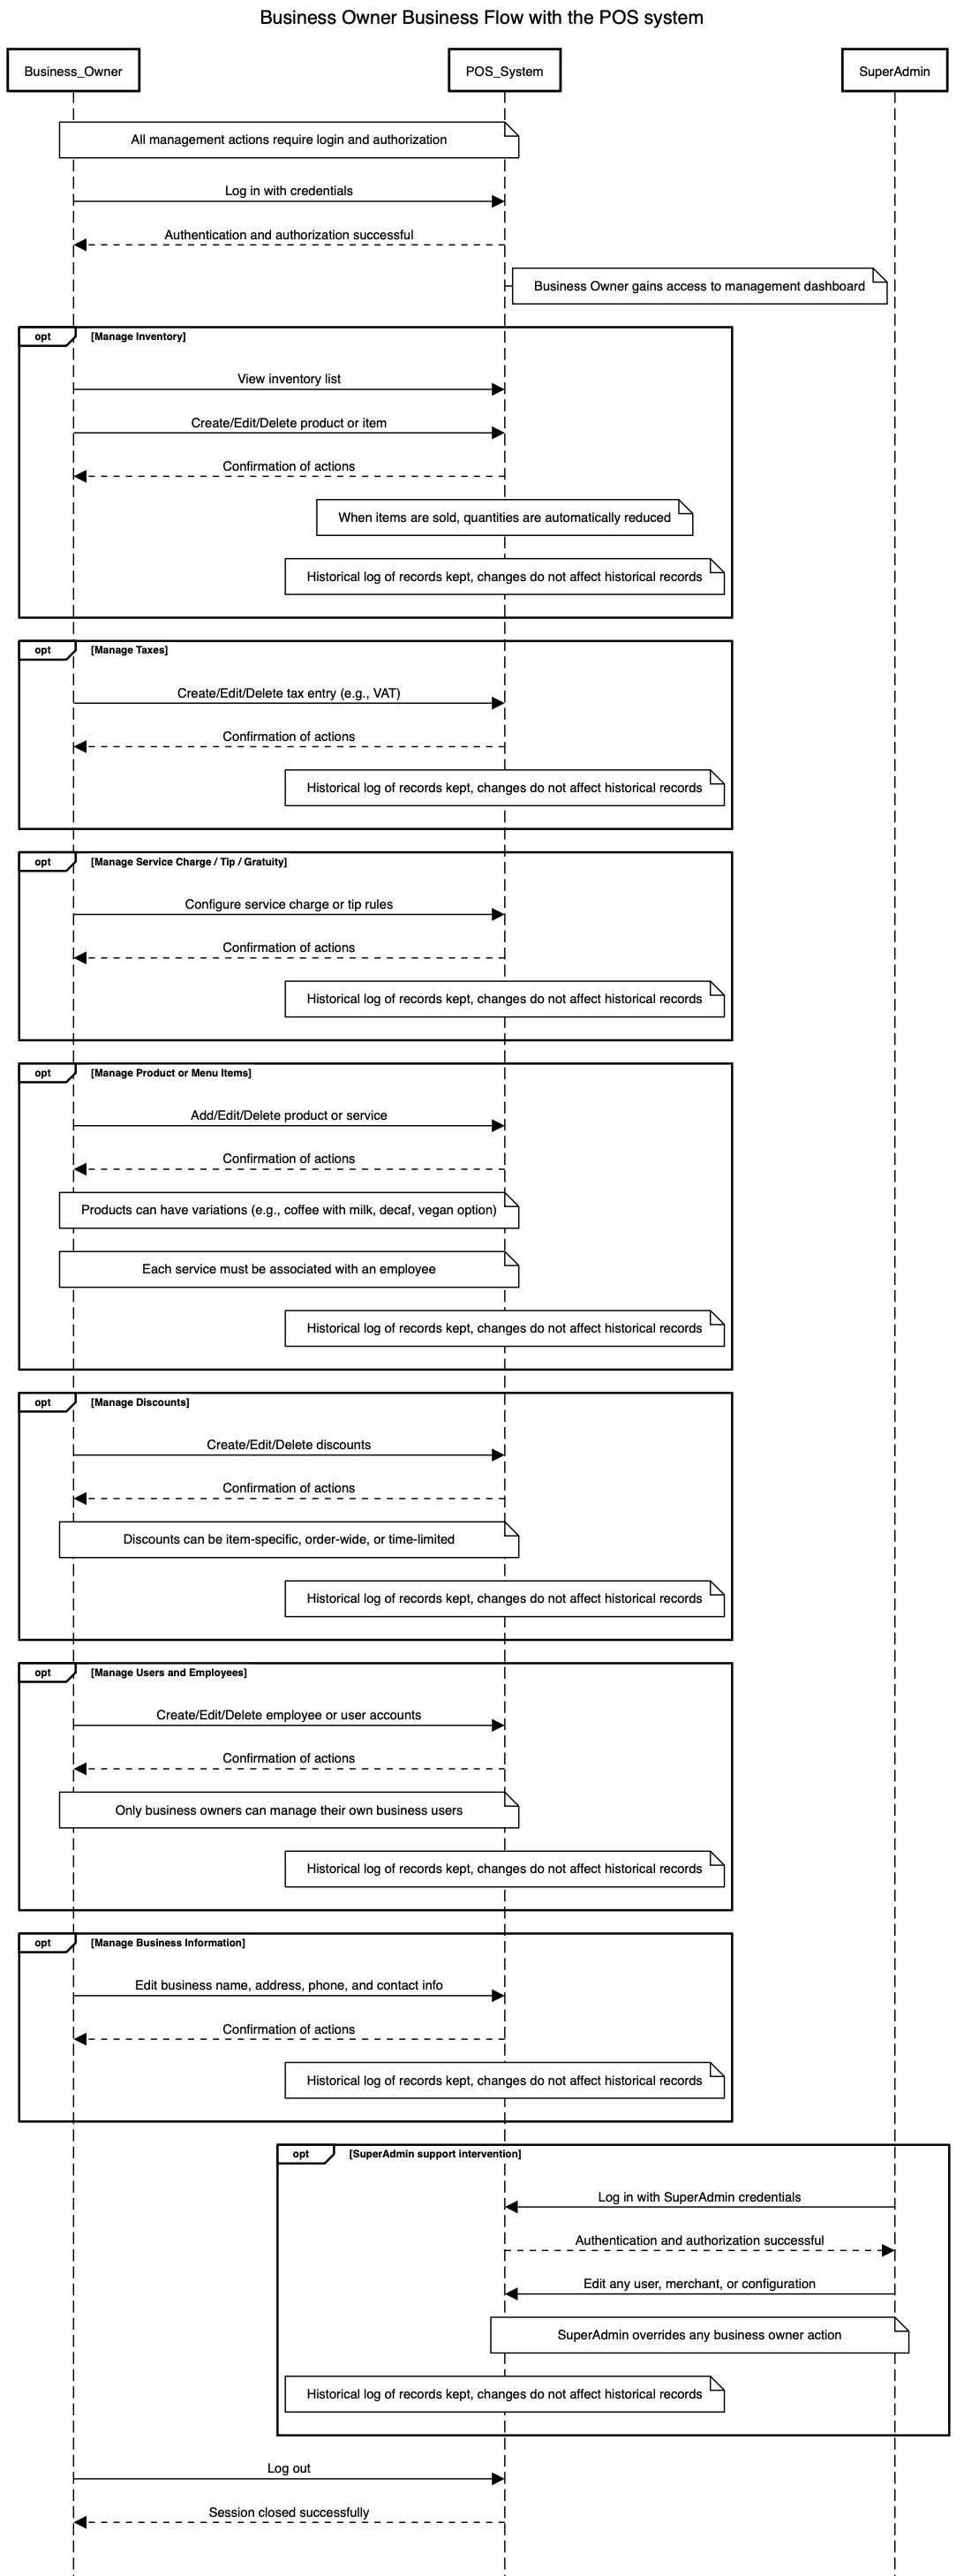
\includegraphics[scale=0.22]{graphics/business owner.png}
    \caption{Sequence diagram displaying possible business owner management actions}
    \label{figures:sequence_business_owner}
\end{figure}




\section{UI wireframes}
To better visualize how the system would look, we can make wireframes. Wireframes can also help to figure out what APIs we need.

\begin{figure}[H]
    \centering
    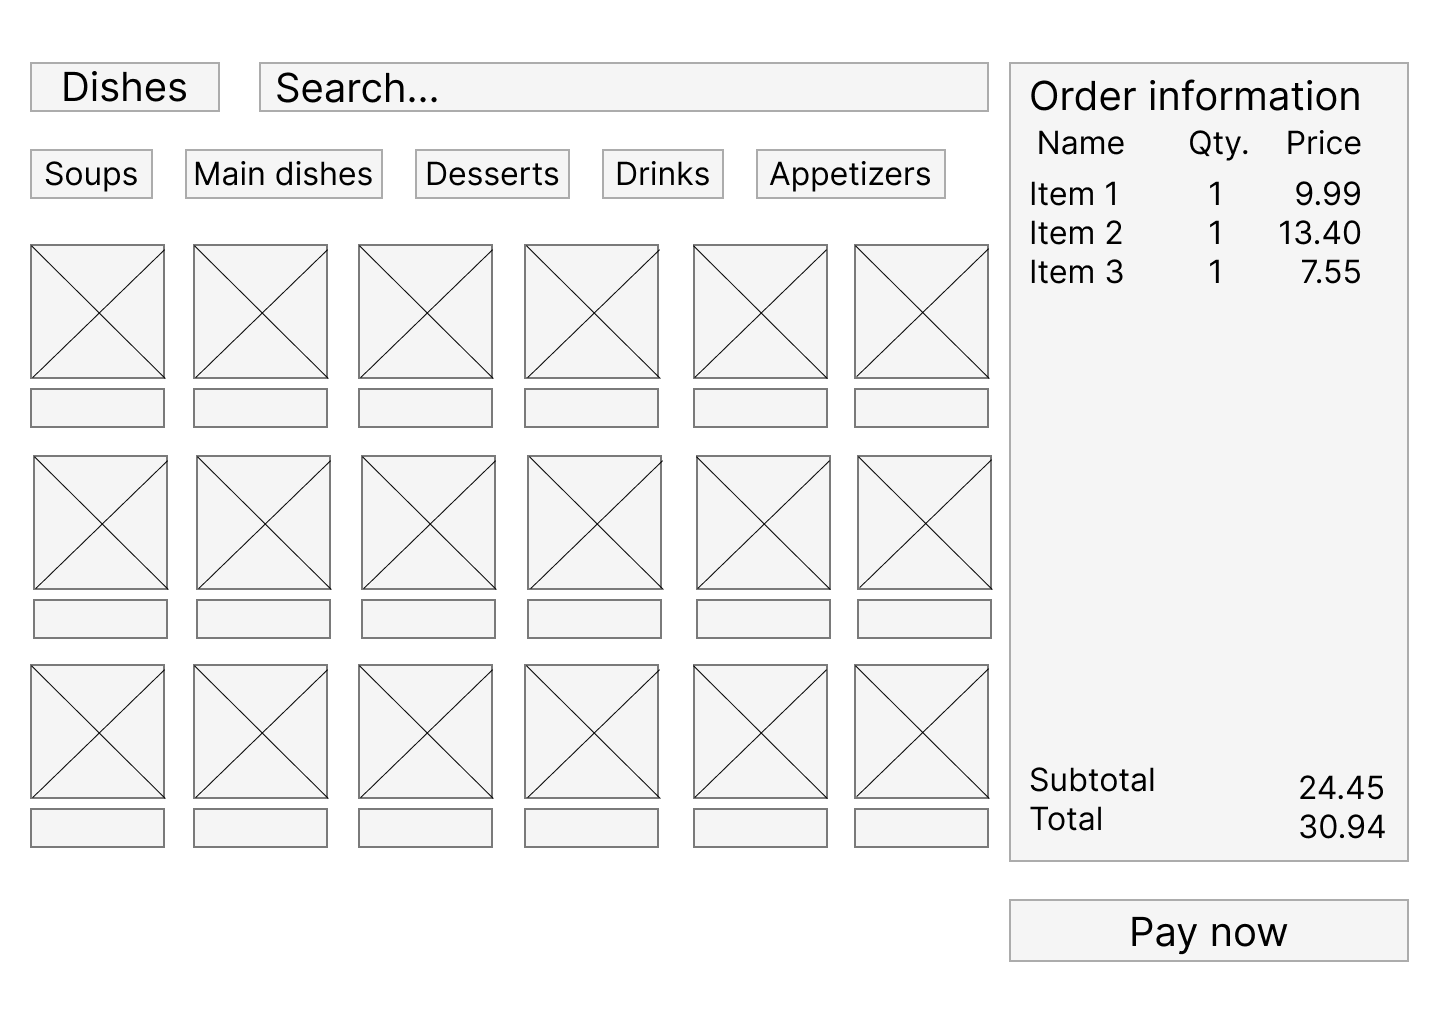
\includegraphics[width=1\linewidth]{ProductSelection.png}
    \caption{A wireframe showing the selection of products when creating an order}
    \label{fig:wireframe_product_selection}
\end{figure}

The wireframe in Figure \ref{fig:wireframe_product_selection} shows the product selection page for order creation. The user can search for dishes by selecting the category (soups, drinks, etc.) and choosing one of the displayed items. It is also possible to search for dishes by typing in at least a part of the name of the wanted item. The selected items show up in the order information section along with the quantity selected and price. At the bottom of the order information section the subtotal and total of the whole order are displayed. Below there is a button \enquote{Pay now} that lets the user proceed to the payment for this order.


\section{Package diagram}


\begin{figure}[H]
    \centering
    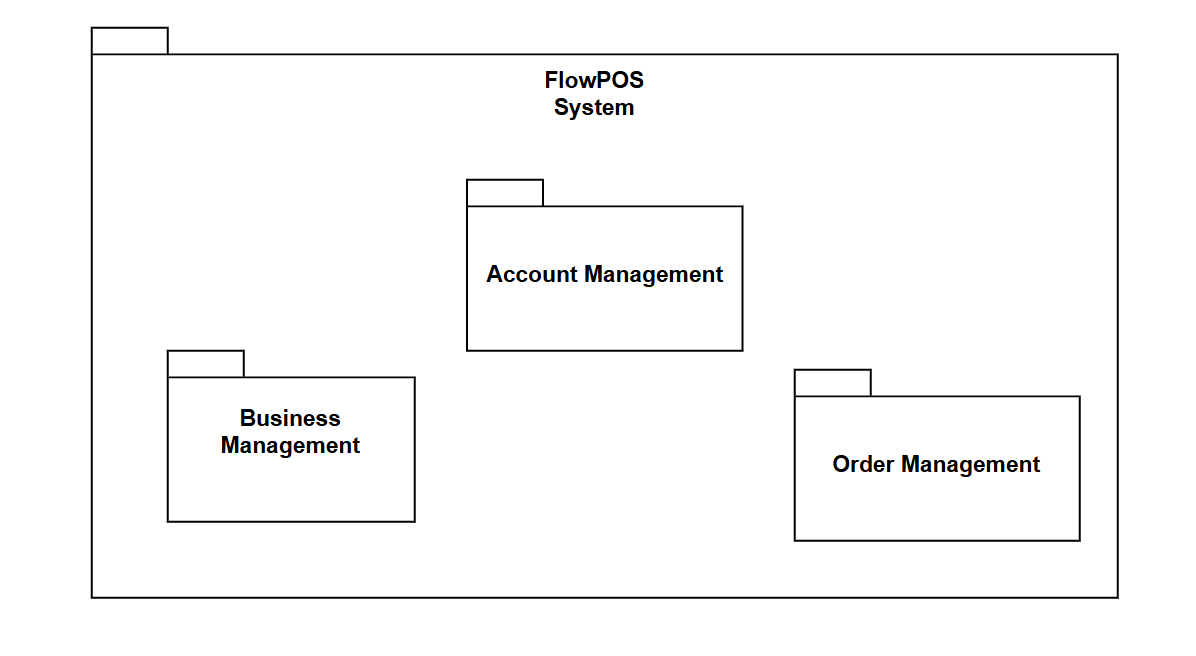
\includegraphics[width=0.9\textwidth]{graphics/Package1.png}
    \caption{FlowPOS Main Package Diagram}
    \label{fig:package1}
\end{figure}

This top-level diagram represents the overall architecture of the FlowPOS system. 
It is divided into three main functional packages: \textbf{Business Management}, \textbf{Account Management}, and \textbf{Order Management}. 
Each package encapsulates related responsibilities and can evolve independently. 
The diagram provides a clear, business-oriented view of the system’s structure and how its major modules are organized.

\subsection{Business Management Package}

\begin{figure}[H]
    \centering
    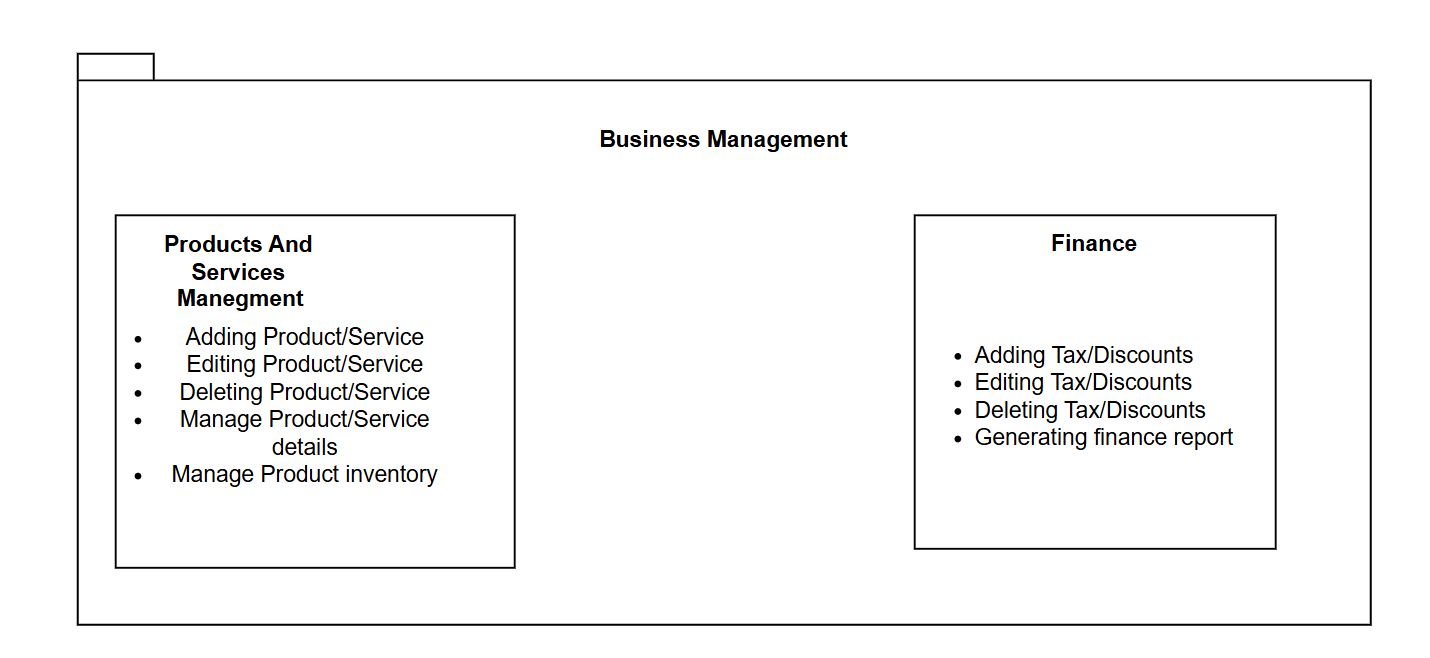
\includegraphics[width=0.9\textwidth]{graphics/Package2.png}
    \caption{Business Management Package}
    \label{fig:package2}
\end{figure}

The \textbf{Business Management} package handles all aspects of products, services, pricing, and financial configurations. 
It is divided into two subpackages:
\begin{itemize}
    \item \textbf{Products and Services Management} – focuses on adding, editing, and maintaining products and services, as well as managing inventory.
    \item \textbf{Finance} – deals with taxes, discounts, and financial reporting.
\end{itemize}
Together, they ensure that the POS system has accurate and up-to-date product and pricing information.

\subsection{Account Management Package}

\begin{figure}[H]
    \centering
    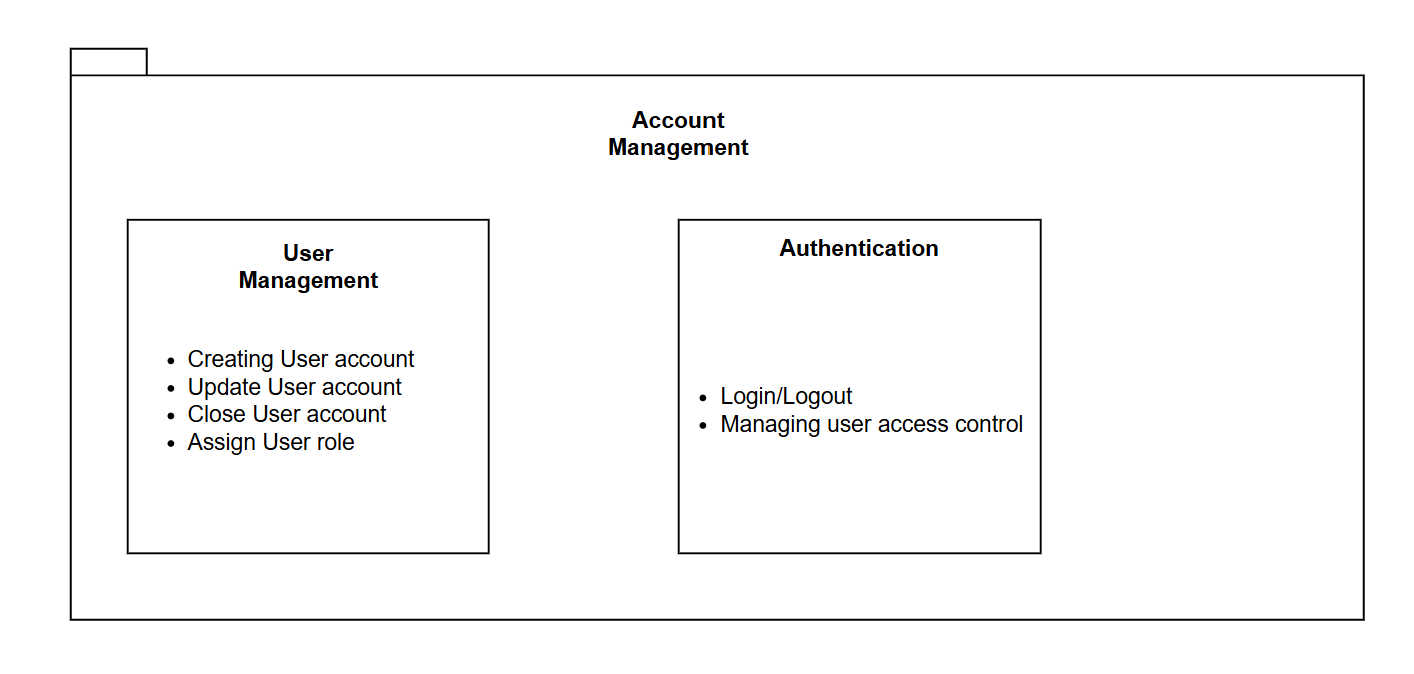
\includegraphics[width=0.9\textwidth]{graphics/Package3.png}
    \caption{Account Management Package}
    \label{fig:package3}
\end{figure}

The \textbf{Account Management} package covers user and role administration, including creating accounts, editing permissions, and assigning roles. 
It ensures secure access control and supports different user types (e.g., cashier, manager, admin). 
This package provides the foundation for authentication and authorization across the system.

\subsection{Order Management Package}

\begin{figure}[H]
    \centering
    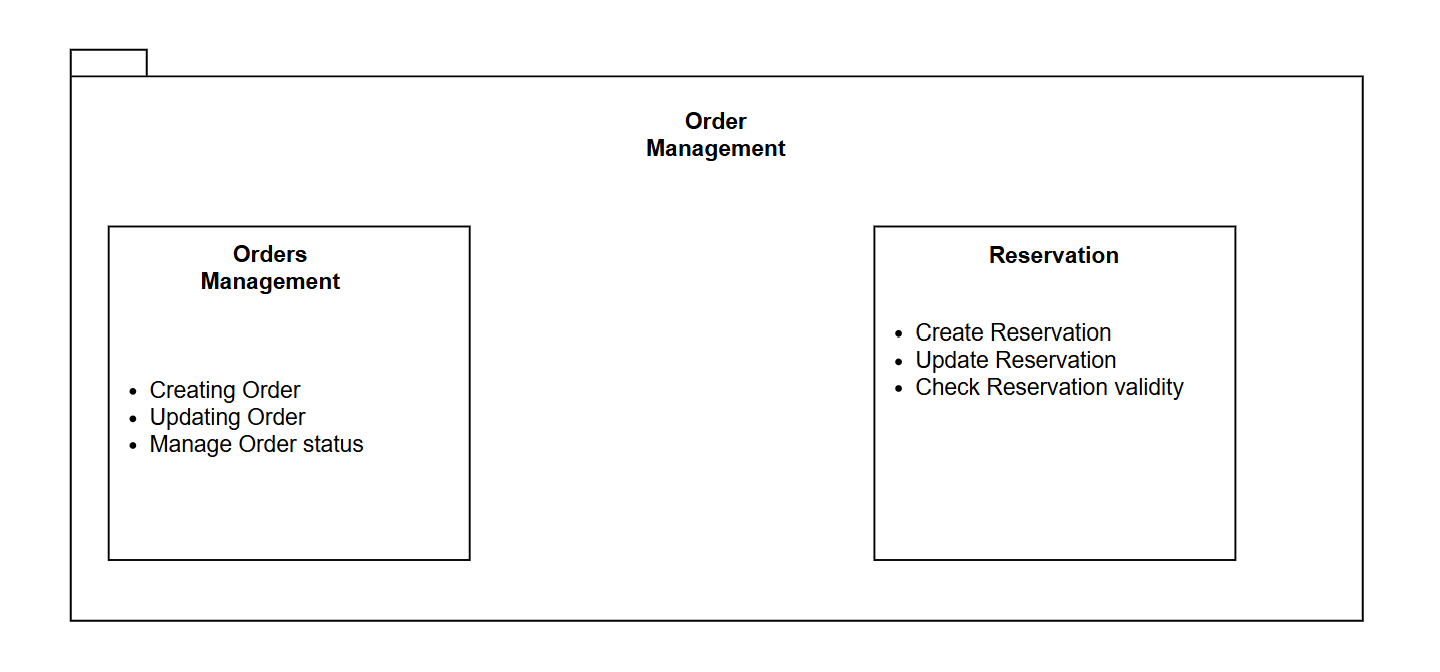
\includegraphics[width=0.9\textwidth]{graphics/Package4.png}
    \caption{Order Management Package}
    \label{fig:package4}
\end{figure}

The \textbf{Order Management} package focuses on the sales and reservation processes within FlowPOS. 
It includes two subpackages:
\begin{itemize}
    \item \textbf{Orders Management} – responsible for creating, updating, and tracking customer orders and their statuses.
    \item \textbf{Reservation} – manages service reservations, allowing users to create, edit, and validate booking details.
\end{itemize}
This module forms the operational core of the POS system, where transactions and customer interactions occur.
% jei daugiau negu 10, tai darom persmulkiai
% 1. Package diagrams.
%    Acount class
%    Business Class   
%    
%  NO INT on price/currency 
%  Money class
\section{Data model}
One of the main challenges within this domain is having a data model that would allow us to persist certain entities in such a way that would allow us to calculate various receipts, reports, and metrics from historic data no matter how the entities change over the course of their lifetime.

To address this problem, we will use the entity lifecycle mechanism. Selected entities, which need their historic changes persisted, will inherit from \enquote{LifecycledEntity}. A lifecycled entity will only have one valid revision at a time; this revision will be identified by the row which has the identifier of the entity, a set \enquote{validFrom} value, and a \textbf{null} \enquote{validTo} column. This means that:
\begin{itemize}
    \item \textbf{On entity creation:} we persist a row with initial values for the entity and a \enquote{validFrom} column value of the timestamp at the time of creation and a \enquote{validTo} value of \textbf{null}.
    \item \textbf{On entity modification:} in a single transaction we first set \enquote{validTo} on the currently active revision to the current timestamp, then persist a new row with the modified entity values, a \enquote{validFrom} value set to the current timestamp (the same value as \enquote{validTo} from the previous revision), and a \enquote{validTo} value set to \textbf{null}.
    \item \textbf{On entity deletion:} we set the \enquote{validTo} column value on the currently active revision to the current timestamp.
\end{itemize}

\begin{figure}[H]
    \centering
    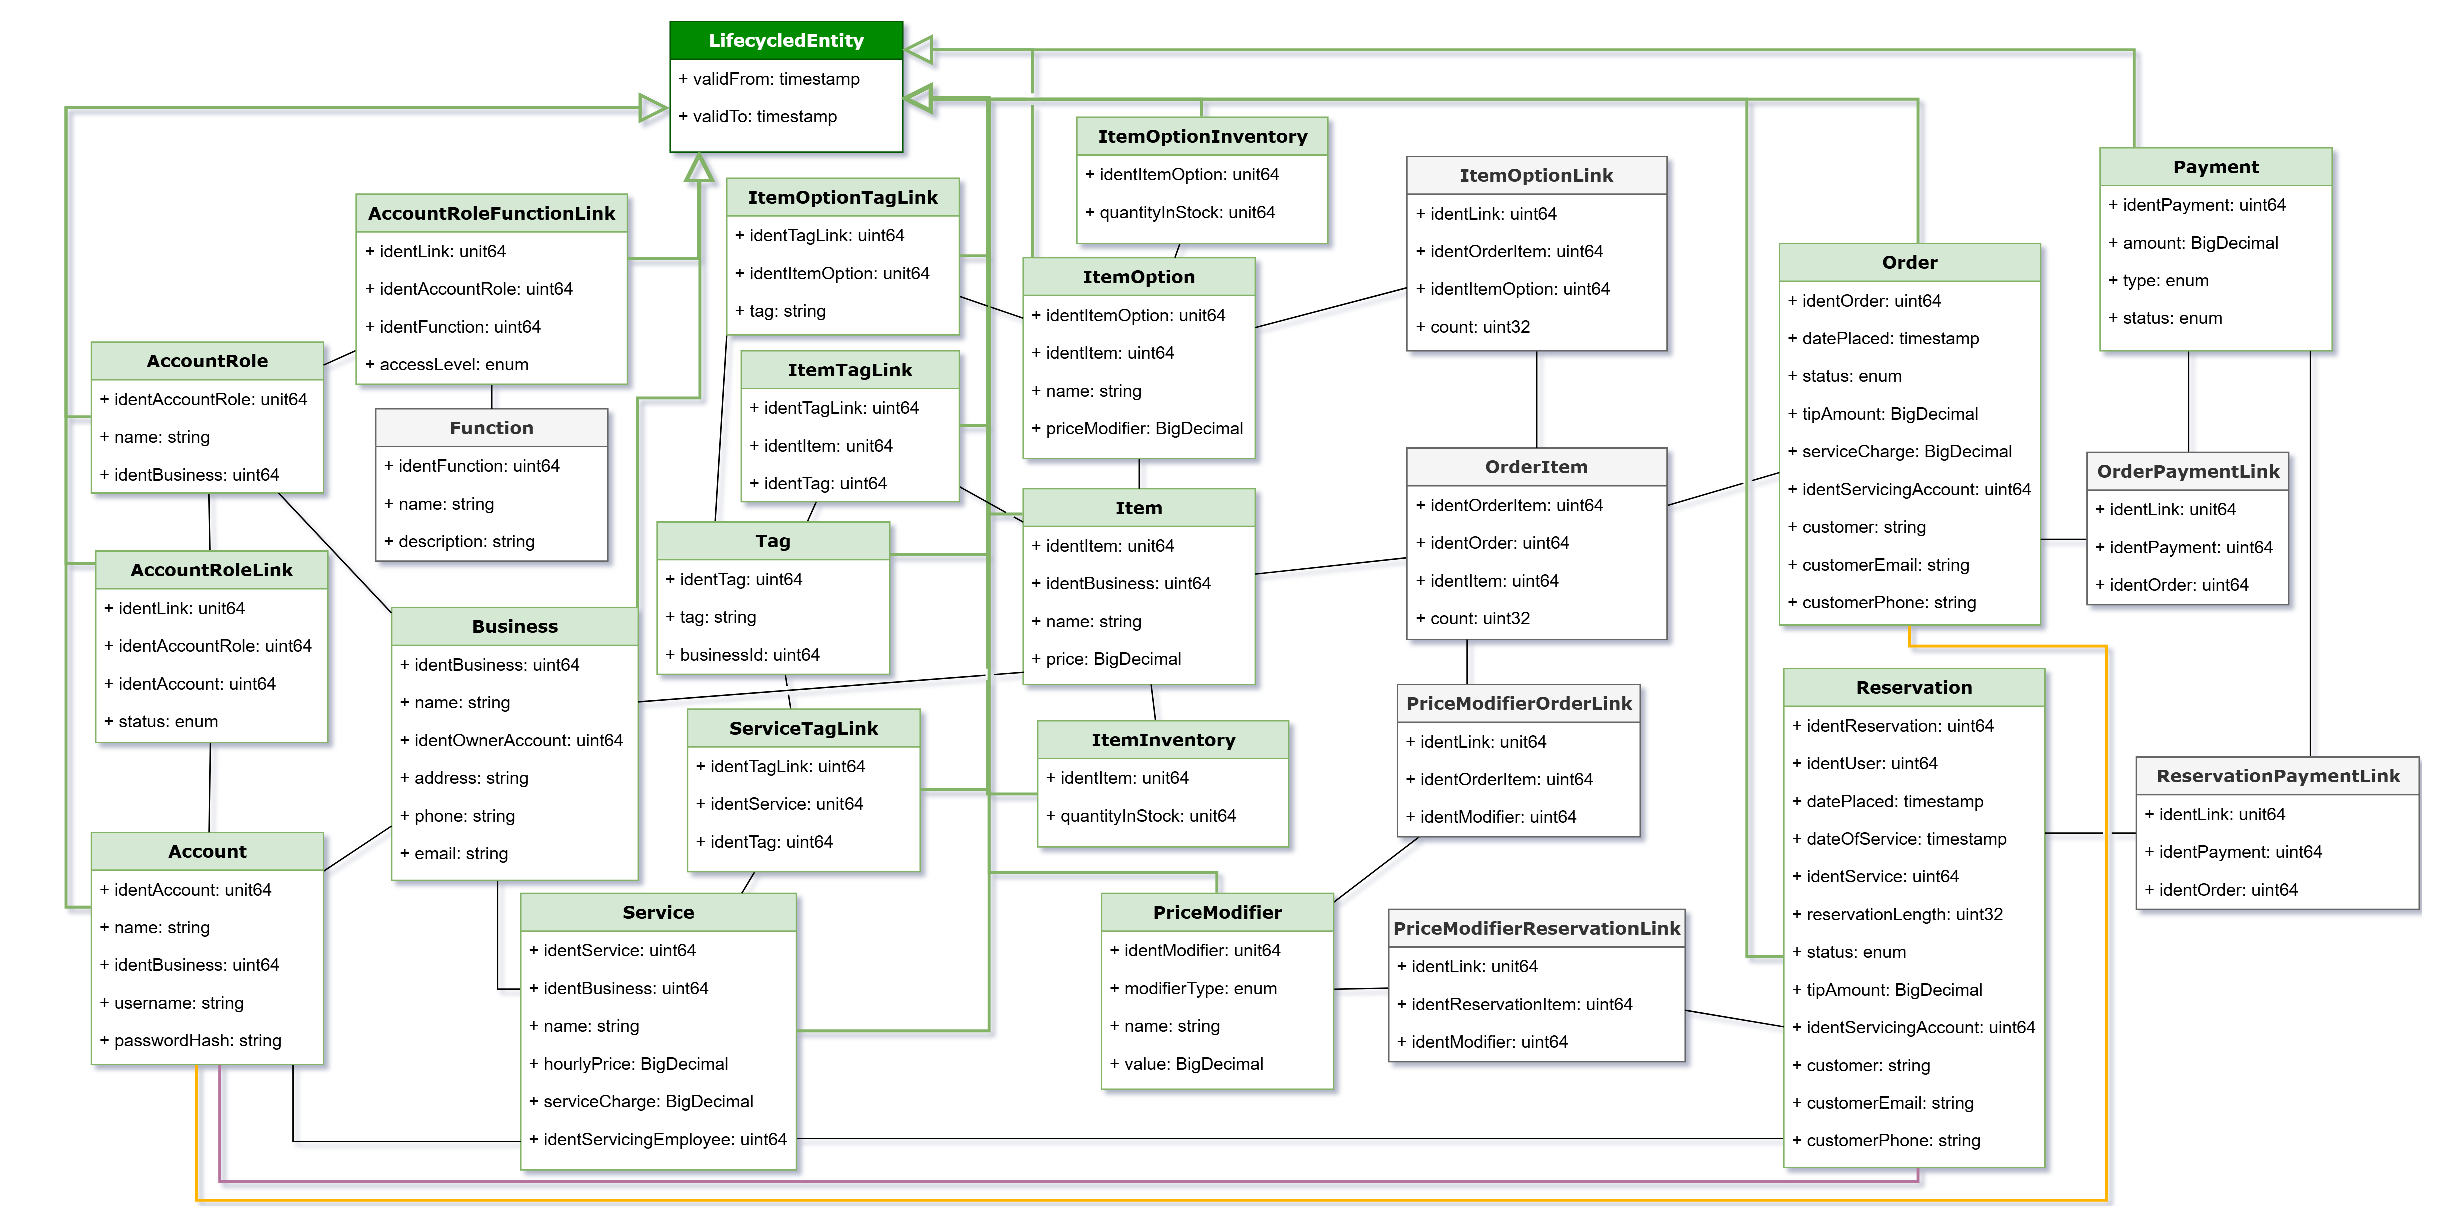
\includegraphics[width=1\linewidth]{data_model.drawio.pdf}
    \caption{Caption}
    \label{fig:data_model}
\end{figure}

% ar reikia UML composition/aggregation?
The diagram in Fig. \ref{fig:data_model} shows the main entities within our data model as well as which entities will be lifecycled (highlighted in green).

\begin{itemize}
    \item \textbf{AccountRole:} Main entity for authorization. Account roles can be created or modified by business owners. Business owners will always have the role BusinessOwner assigned. The created roles can be assigned functions (Order creation, order view, etc.) which are mapped to specific functionalities within the system. Account roles will be used when looking up wether the executing user can execute a certain function.
    \item \textbf{Function:} These represent the functions within the system.
    \item \textbf{AccountRoleFunctionLink:} Used to assign specific functions to a specific role and a access level (view initiate) for that function.
    \item \textbf{Account:} Account for a user of the system. The identBusiness field may only be unset (0) when an account is created to register a new business. Accounts created for a specific business will always have a business identifier set.
    \item \textbf{AccountRoleLink:} Used to configure Account - AccountRole relationships. Will have a possible status of: 
    \begin{itemize}
        \item Active - the account currently has the role assigned and can access related functions;
        \item Suspended - the account currently has the role assigned, but accress to related functions is \textbf{temporarily} suspended;
        \item Deactivated - the account role assignment is \textbf{permanently} disabled (a new assignment would need to be created to assign the same role again).
    \end{itemize}
    \item \textbf{Bussiness:} Entity representing a registered business. May only have a single owner.
    \item \textbf{Item:} An item that can be registered to a specific business which can be used to form orders.
    \item \textbf{ItemInventory:} A separate table (although can me combined with Item) to \textbf{OPTIONALLY} track item inventory in the system. If a row does not exist for a specific Item that means the item's quantity is not being tracked.
    \item \textbf{ItemOption:} An item specific additional option (Almond milk on coffee). The price modifier will be a flat value which can either be negative or positive in order to indicate wether the item price will be reduced or increased by the set value, or unmodified if set to 0.
    \item \textbf{ItemOptionInventory:} A separate table (although can me combined with ItemOption) to \textbf{OPTIONALLY} track item inventory in the system. If a row does not exist for a specific ItemOption that means the ItemOptions's quantity is not being tracked.
    \item \textbf{ItemOptionLink:} Used to add item options to an item in a specific order. Item options can only be assigned/removed to/from an order if the order is not in a final state (Confirmed, Completed, Refunded, etc.).
    \item \textbf{Tag:} Tags are a business specific way to categorize Items, ItemOptions and Services. They are mainly used to query the aforementioned entities.
    \item \textbf{ItemTagLink:} Relation for Items and Tags.
    \item \textbf{ItemOptionTagLink:} Relation for ItemOptions and Tags.
    \item \textbf{SericeTagLink:} Relation for Services and Tags.
    \item \textbf{PriceModifier:} Entity for handling discounts and taxes. The modifier type will be used to identify wether the modifier is a \textbf{flat} discount/tax or a \textbf{percentage} based one. The identifier will advise on how we should use the value to calculate the final price of an item/reservation.
    \item \textbf{PriceModifierOrderLink:} Used to add a discount/tax o a specific item in a specific order.
    \item \textbf{PriceModifierReservationLink:} Used to add a discount/tax o a specific item in a specific reservation.
    \item \textbf{Service:} A service that may be offered by a specific business (haircut, massage, etc.). Contains the hourly price which will be used to calculate the final price of the reservation, the service charge and identifier for the account of the employee will carry out the service.
    \item \textbf{Reservation:} An entity representing a booking for a certain service.
    \item \textbf{Order:} The entity representing an order of items from a specific business.
    \item \textbf{OrderItem:} A way to assign items to an order. Items may only be assigned/removed to/from an order if the order is not in a final state (Confirmed, Completed, Refunded, etc.).
    \item \textbf{Payment:} The entity used to persist payment details for a order/reservation. May be a cash/card/gift card payment.
    \item \textbf{OrderPaymentLink:} Used to assign payments to an order (may be multiple payments per order if check was split).
    \item \textbf{ReservationPaymentLink:} used to assign payments to reservations (may be multiple payments per order if check was split).
\end{itemize}

\section{API Contracts}

\subsection{HTTP requests}

All detailed API specifications are available in the Swagger yaml file. This file is located in the main GitHub repository of this project.

\subsubsection{Account Management APIs}
\textbf{Account:}\\
% /account
%     POST
%     GET
% 
% /account/login
%     POST
\hspace*{1em}\textbf{/account}\\
\hspace*{2em}\textbf{POST} Description: Create worker account\\
\hspace*{2em}\textbf{GET} Description: Get all accounts (with pagination)\\

\hspace*{1em}\textbf{/account/login}\\
\hspace*{2em}\textbf{POST} Description: Log in to account\\

\hspace*{1em}\textbf{/account/\{id\}}\\
\hspace*{2em}\textbf{GET} Description: Get account information\\
\hspace*{2em}\textbf{DELETE} Description: Delete an account\\


\textbf{AccountRole:}\\
\hspace*{1em}\textbf{/account/role}\\
\hspace*{2em}\textbf{POST} Description: Create a new role for business\\
\hspace*{2em}\textbf{GET} Description: Get all roles for current business\\

\hspace*{1em}\textbf{/account/role/\{roleId\}}\\
\hspace*{2em}\textbf{GET} Description: Get details of a specific role\\
\hspace*{2em}\textbf{PUT} Description: Update role details\\
\hspace*{2em}\textbf{DELETE} Description: Delete a role\\

\hspace*{1em}\textbf{/account/role/\{roleId\}/function}\\
\hspace*{2em}\textbf{POST} Description: Assign a function to a role with specified access level\\
\hspace*{2em}\textbf{GET} Description: Get all functions assigned to a specific role\\

\hspace*{1em}\textbf{/account/\{accountId\}/role}\\
\hspace*{2em}\textbf{POST} Description: Assign a role to an account\\
\hspace*{2em}\textbf{GET} Description: Get all roles assigned to an account\\

\hspace*{1em}\textbf{/account/\{accountId\}/role/\{roleId\}}\\
\hspace*{2em}\textbf{PUT} Description: Update the status of a role assigned to an account\\


\subsubsection{Function API}\\

\textbf{Function:}\\
\hspace*{1em}\textbf{/function}\\
\hspace*{2em}\textbf{GET} Description: Get all available system functions\\


\subsubsection{Business Management APIs}\\

\textbf{Business:}\\
\hspace*{1em}\textbf{/business}\\
\hspace*{2em}\textbf{POST} Description: Create business\\
\hspace*{2em}\textbf{GET} Description: Get all businesses user has access to\\

\hspace*{1em}\textbf{/business/\{id\}}\\
\hspace*{2em}\textbf{GET} Description: Get business information\\

\textbf{Item:}\\
\hspace*{1em}\textbf{/item}\\
\hspace*{2em}\textbf{POST} Description: Create item for current business\\
\hspace*{2em}\textbf{GET} Description: Get all items of current business\\

\hspace*{1em}\textbf{/item/\{id\}}\\
\hspace*{2em}\textbf{GET} Description: Get item by id\\
\hspace*{2em}\textbf{PUT} Description: Edit item\\
\hspace*{2em}\textbf{DELETE} Description: Delete an item\\

\textbf{ItemOption:}\\
\hspace*{1em}\textbf{/item-option}\\
\hspace*{2em}\textbf{POST} Description: Create a new item option\\
\hspace*{2em}\textbf{GET} Description: Get all item options\\

\hspace*{1em}\textbf{/item-option/\{id\}}\\
\hspace*{2em}\textbf{GET} Description: Get item option by id\\
\hspace*{2em}\textbf{PUT} Description: Update an item option\\
\hspace*{2em}\textbf{DELETE} Description: Delete an item option\\



\textbf{PriceModifier:}\\
\hspace*{1em}\textbf{ } /\\
\hspace*{2em}Description: 

\subsubsection{Order Management APIs}

\textbf{Order:}\\
\hspace*{1em}\textbf{POST} /\\
\hspace*{2em}Description: Create a new order

\hspace*{1em}\textbf{GET} /\\
\hspace*{2em}Description: Get all orders

\hspace*{1em}\textbf{GET} /\\
\hspace*{2em}Description: Get order by id

\hspace*{1em}\textbf{PUT} /\\
\hspace*{2em}Description: Update order details (status, etc.)

\hspace*{1em}\textbf{POST} /\\
\hspace*{2em}Description: Add an item to an existing order

\hspace*{1em}\textbf{GET} /\\
\hspace*{2em}Description: Get all items in an order

\hspace*{1em}\textbf{PUT} /\\
\hspace*{2em}Description: Update an item in an order

\hspace*{1em}\textbf{DELETE} /\\
\hspace*{2em}Description: 

\hspace*{1em}\textbf{POST} /\\
\hspace*{2em}Description: 

\hspace*{1em}\textbf{POST} /\\
\hspace*{2em}Description: 

\hspace*{1em}\textbf{GET} /\\
\hspace*{2em}Description: 

\hspace*{1em}\textbf{DELETE} /\\
\hspace*{2em}Description: 

\textbf{Service:}\\
\hspace*{1em}\textbf{ } /\\
\hspace*{2em}Description: 

\textbf{Reservation:}\\
\hspace*{1em}\textbf{ } /\\
\hspace*{2em}Description: 

\subsubsection{Payment API}

\textbf{Payment:}\\
\hspace*{1em}\textbf{ } /\\
\hspace*{2em}Description: 


\subsection{HTTP responses}
\hspace*{1em}200 Ok\\
\hspace*{2em}\textbf{Description:} Response to a successful GET, PUT, PATCH, DELETE or POST that doesn't result in a creation.\\
\hspace*{1em}201 Created\\
\hspace*{2em}\textbf{Description:} Response to a POST that results in a creation.\\
\hspace*{1em}204 No Content\\
\hspace*{2em}\textbf{Description:} Response to a successful request that won't be returning a body.\\
\hspace*{1em}304 Not Modified\\
\hspace*{2em}\textbf{Description:} Indicates that the resource has not been modified since the version specified by the request headers If-Modified-Since or If-None-Match.

\subsection{HTTP error codes}
\hspace*{1em}Client:\\
\hspace*{2em}400 Bad Request\\
\hspace*{3em}\textbf{Description:} The request is malformed, wrong parameters or wrong API invocation\\
\hspace*{2em}401 Unauthorized\\
\hspace*{3em}\textbf{Description:} When no or invalid authentication details are provided.\\
\hspace*{2em}403 Forbidden\\
\hspace*{3em}\textbf{Description:} When authentication succeeded but authenticated user doesn't have permission to access the resource in question.\\
\hspace*{2em}404 Not Found\\
\hspace*{3em}\textbf{Description:} When a non-existent resource is requested.\\
\hspace*{2em}405 Method not supported\\
\hspace*{3em}\textbf{Description:} When given HTTP verb is not supported for such endpoint.\\
\hspace*{2em}422 Unprocessable Entity\\
\hspace*{3em}\textbf{Description:} Used for validation errors.
   
\hspace*{1em}Server:\\
\hspace*{2em}500 Internal Server Error\\
\hspace*{3em}\textbf{Description:} A generic error message, given when an unexpected condition was encountered, and no more specific message is suitable.\\
\hspace*{2em}502 Bad Gateway\\
\hspace*{3em}\textbf{Description:} The server was acting as a gateway or proxy and received an invalid response from the upstream server.\\
\hspace*{2em}503 Service Unavailable\\
\hspace*{3em}\textbf{Description:} The server cannot handle the request.\\
\hspace*{2em}504 Gateway Timeout\\
\hspace*{3em}\textbf{Description:} The server was acting as a gateway or proxy and did not receive a timely response from the upstream server.

% Catering:
%  Client
%   Get receipt
%   Pay using cash, bank or gift card

%  Waiter
%   Create reservations
%   Check reservations,
%   Check taken/free tables
%   Mark tables as taken/free
%   Create order, add some special requests
%   See order status
%   Change existing orders
%   Create receipt
%   Add discount/tip to order

%  Kitchen staff
%   See order
%   Mark order as done

% Beauty:
%  Client
%   Give personal info
%   Get SMS confirmation
%   Pay using cash, bank or gift card

%  Receptionist
%   Check time slots for services
%   Check reservations
%   Create reservations
%   Mark times for services as taken/free
%   Change reservations
%   Add discount/tip to order

\end{document}
